% =====================================================================
% Part III -- Endogenous Coupling and Exotypes.  Draft 2026-08-06 (claude-14).
%
% Scope per Joe, 2026-08-06: Part III explains the exotype layer and reports
% what the search found AT THE END.  The EFE miner -- the apparatus that did the
% searching -- moves to a supplement: it is a tool, not a theory of MetaCAs.
% Update 2026-08-08 (fable): the research question is closed by deterministic
% measurements (TN-part-iii-endogenous-ruling.md, incl. its retraction
% addenda; scripts none_label_check, lstar_tau_measure,
% hetfixed_sheet_reference, boundary_invasion_rescue, boundary_blast,
% morphology_default_check).  Section order follows the discovery order:
% gate -> layer -> vocabulary -> scope -> three outcomes -> closure (last,
% with the combined two-interventions figure).
%
% Labels referenced here that exist in draft7.tex: sec:object, eq:prop,
% sec:classification, sec:census, sec:full-census, sec:gain, part:core.
% =====================================================================

\part{Exotypes}
\label{part:endogenous}

\noindent In Part~II the gain of the phenotype-to-genotype loop is a parameter
we set, and the gate of \secref{sec:endogenous-gain} made the firing
condition a function of the lattice while the operator remained a property of
the run. This part takes the remaining step: the operator itself becomes a
property of the cell.

Its findings, in order. When the operator becomes per-cell state, adopted
between neighbours under a selection rule, three outcomes occur at the tested
parameters: the changing phase (sites whose phenotypes continue to update) eliminates the frozen phase (sites whose phenotypes remain unchanged for fifteen steps), the frozen phase
takes over, or the two persist together for the full horizon. No locally
computable quantity we tested ranks operators well enough to find the third
outcome from within a run. A local intervention built to protect it---cells in
uniform surroundings copying operators from phase boundaries---accelerates
the freezing instead. Undirected noise does prevent freezing, but what it
holds looks different: a foam of small frozen islands amid changing
surroundings (Figure~\ref{fig:interventions}), against the extended frozen
and changing regions of the found configuration
(Figure~\ref{fig:exo-lavalamp}); the measured difference is frozen
fraction, $0.3$ against $0.08$. Finally, with adoption
switched off, none of thirty control runs freezes or dies: the frozen
endpoints are an effect of the adoption rule at high precision, not of the
lattice underneath. Two probes directed by the literature sharpen both
findings: the freeze is nucleation-limited (an established frozen domain
invades, yet the frozen phase never arises from developed churn), and a
one-sided rule that writes only into long-settled cells holds a mixed state
at a sixth of the dose of its randomly placed control --- placement carries
information after all, once the trigger is one-sided.

\section{The Gate Sets the Timing of Rewrites; the Exotype Sets Their Content}
\label{sec:exotype-intro}

The gate of \secref{sec:endogenous-gain} chooses \emph{when} an operator
fires. It does not choose \emph{which}: there the pair of constituents is fixed, and the
predicate selects between them; the permutation $\sig$ supplying the rewriting is
a property of the run.  Each
cell carries its own propagator, drawn from a small named vocabulary and
transmitted between neighbours, so the operator acting at a site becomes part of
the local state.

Whether such a lattice can find its own operating point, using only
quantities available to it at runtime, is the question the remainder of the
part answers. The instrument behind every measurement so far---causal reach,
computed by forking the run and perturbing a twin---is not such a quantity:
no system can fork itself, and reach measures causal propagation rather than
dynamical regime, so it would not by itself say where the system should
arrive.

\section{The Exotype Is a Structured Mutation Operator}
\label{sec:exotype-layer}

An \emph{exotype} is a per-cell assignment of a propagator. The vocabulary is a
set of named permutations $\sig$; the grid holds one name per site; and the
names are transmitted between neighbouring sites by a local policy. Nothing in
the vocabulary is new to this paper---each name denotes a member of the family
Equation~\eqref{eq:prop} defines---but the assignment is new, because $\sig$ has
until now been a property of a run rather than of a cell.

The transition is one elementary write. At a site whose genotype is the
eight-bit rule $g$, with $\sig$ the propagator the site currently carries, a
coordinate $k \in \{0,\dots,7\}$ is drawn uniformly at each step and
%
\begin{equation}
  g'\bigl(\sig(k)\bigr) \;=\; \neg\, g(k),
  \label{eq:exotype-write}
\end{equation}
%
with $g$ unchanged elsewhere. Comparing this with \secref{sec:object}: the
simultaneous operator $P_\sig$ applies Equation~\eqref{eq:exotype-write} at all
eight coordinates at once, and the spatial experiments of Part~I place its
elementary writes inside the two-layer automaton. The exotype layer is that same
elementary write, drawn one coordinate at a time, with $\sig$ read from the cell
rather than from the run.

Three properties matter for what follows. The exotype edits the rule, not
how the rule is applied: $\sig$ selects a write address inside the genotype,
and the term \emph{propagator} (Part~I) names this movement of bits through
the truth table, not any propagation of phenotype state. When $\sig$ is the
identity the transition is a point mutation; for every other $\sig$ the read
and write addresses differ, so the operation transfers inverted information
from one truth-table entry to another---a locally varying, \emph{structured}
mutation operator whose bias is which bit is rewritten from which. And it
fires at every applied site at every step: the ordinary path, not a rare
perturbation. The exotype grid persists across steps and is transmitted
between sites---inheritance of an acquired modifier, in the sense that a
Baldwin-style argument requires.

The implemented vocabulary is twelve named members of the
$40{,}320$-member family.\phantomsection\label{sec:exotype-vocabulary}%
\phantomsection\label{sec:exotype-scope} Part~I audits it exactly: the
theorem predicts, without any dynamical measurement, how many rules each
member cannot alter, and the prediction agrees in all fourteen implemented
cases, including two controls that are defined but not selectable---an audit
of the vocabulary, not a premise of any result below. The twelve span both
cycle parities and both ends of the fixed-point count, which makes the
layer's behaviour attributable to the exotype mechanism rather than to a
degenerate choice of operator. The boundary this small sample places on the
part's claims is stated with the other limits in \secref{sec:limits}.

\section{Three Outcomes: The Changing Phase Wins, the Frozen Phase Wins, or Neither Does}
\label{sec:exotype-examples}

Supplement~4 records a search over two parameters of the selection rule: the
policy precision $\beta$, which controls how strongly selection concentrates on the lowest-scoring candidate, and epistemic weight $\kappa$, which scales the information-seeking term relative to the goal-directed term. The search was
not endogenous---the apparatus varied the parameters and scored the runs
from outside, and the examples below were located with it operated
interactively, under manual selection among its outputs. (One of its
results bears on what follows: two runtime-computable observables, halting share and change rate,
predict the intrinsic local-compressibility objective well, $R^2 = 0.73$ held out, and damage reach
not at all, $R^2 = 0.02$.) What the search produced is a map: on the
$(\beta,\kappa)$ surface the region of non-zero values of the 250-step search objective is an
L-shaped \emph{ridge}, one arm at low precision, the other at low epistemic
weight, and the three configurations reported below sit on it --- what a
working search would have been expected to return. They establish that the targets of such a search
exist in this substrate; whether the substrate can find them is the question
the last two sections take up.

All three are measured the same way and by a criterion the search never used.
Write a site as \emph{frozen} at time $t$ if its phenotype has been unchanged for
the preceding fifteen steps, and \emph{live} otherwise. A run is \emph{absorbing}
if it reaches a configuration it does not leave again for the remainder of the
run. These are properties of a single
trajectory, requiring no twin run and no external reference; the horizon is the
only free choice, and we report it with every number.

\subsection{At low precision, the changing phase eliminates every frozen region}

At low $\beta$ the lattice is live and stays live (Figure~\ref{fig:exo-bifurcation}). At $\beta = 2$, $\kappa = 0$
the frozen fraction settles at $0.040$ and remains there through $3000$ steps, on
both seeds; the same holds at $\beta = 2$, $\kappa = 0.1$ and at $\beta = 4$ for
$\kappa \in \{0, 0.1, 0.2\}$. No run in this group reaches an absorbing state.

The mechanism is not that frozen regions fail to form. They form and are then
eaten. Over the first three measurement bands at $\beta = 2$, $\kappa = 0$ the
number of frozen domains holds at ten while their mean width collapses from
$9.0$ cells to $3.8$ and then to zero. A constant count with falling width is
boundary retreat: every domain loses territory from both edges at once. Interior
dissolution would look different --- holes opening inside frozen regions would
\emph{raise} the domain count by fragmentation --- and the count never rises.
Live territory invades frozen territory at every boundary simultaneously, and
there is nothing left at the end.

\subsection{At high precision, the frozen phase takes over the lattice}

At high $\beta$ and low $\kappa$ the same contest runs the other way, and the
losing side puts up a fight worth describing. At $\beta = 32$, $\kappa = 0.1$
the lattice carries a dense branching structure through a field of static
stripes, fragmenting the frozen field as it goes: the frozen domain count
\emph{rises} from fifteen to twenty-two over the second measurement band, which
is live territory cutting frozen territory into pieces. It then loses. The
pieces merge, the count falls to two domains of width $124$, and at $t = 1046$
the configuration stops changing and does not change again before the run
ends. Every subsequent row is
byte-identical; the final pattern has density $0.500$, so this is a frozen
pattern rather than a blank sheet.

The second seed absorbs at $t = 460$, and $\beta = 64$ absorbs at $t = 881$ and
$t = 537$. The outcome is seed-robust and the timing is not: absorption time
varies by more than a factor of two at fixed parameters, so differences of that
size between neighbouring $\beta$ carry no information.

\begin{figure}[htbp]
\centering
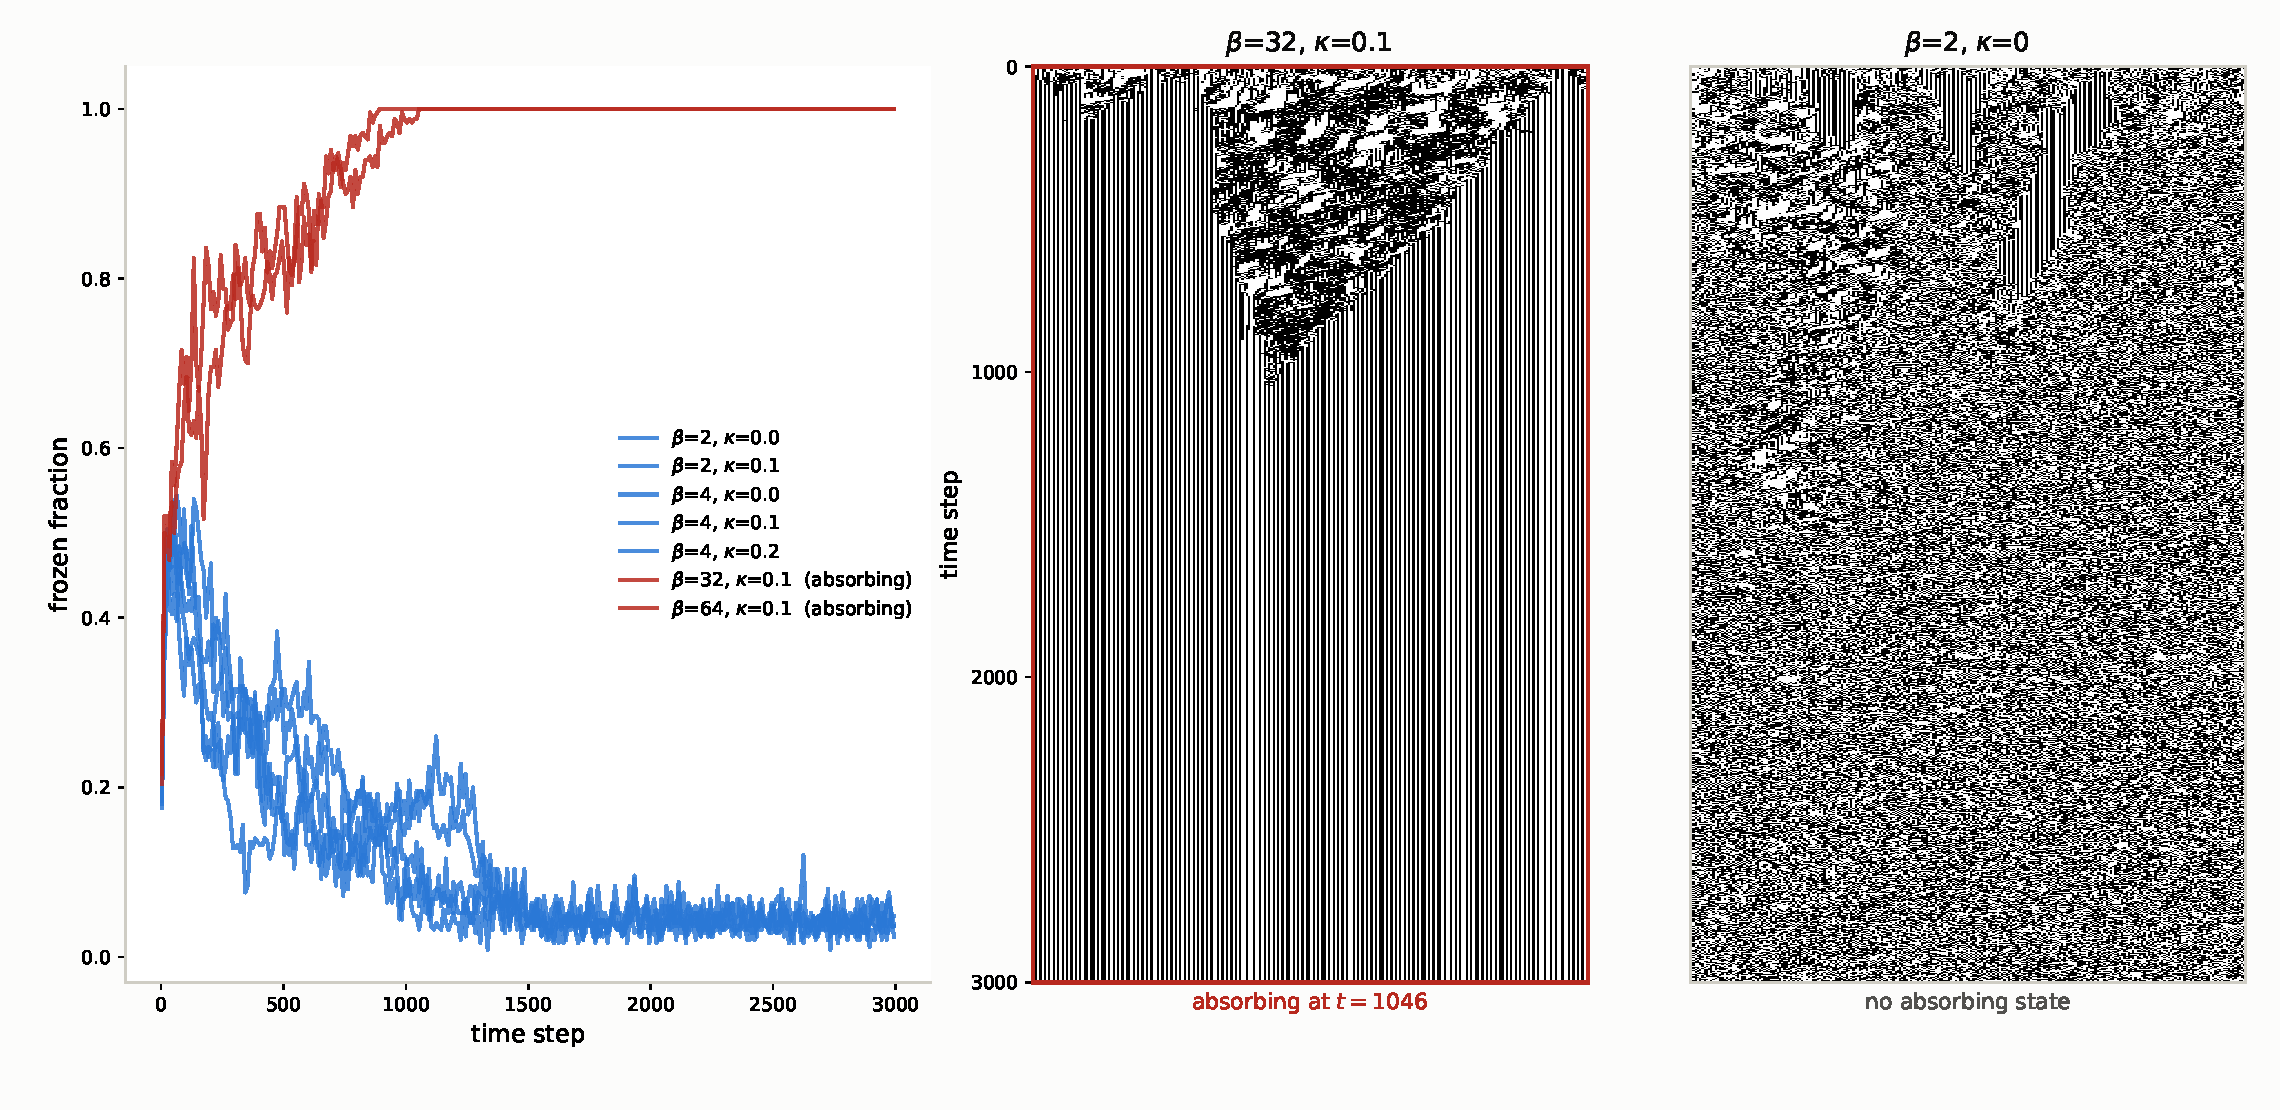
\includegraphics[width=\linewidth]{figures/exo-bifurcation.pdf}
\caption{The two arms of the ridge. Left: frozen fraction against time for the seven
configurations run to $3000$ steps, with the two that reach an absorbing state drawn in
red. The arms separate within the first few hundred steps and do not cross again. Centre
and right: the two extremes as spacetime diagrams --- $\beta = 32$, $\kappa = 0.1$, which
fragments the frozen field for some five hundred steps and is then squeezed out, against
$\beta = 2$, $\kappa = 0$, which erodes the frozen field to nothing and continues. The same
contest, opposite winners.}
\label{fig:exo-bifurcation}
\end{figure}

The two are the same kind of object---both carry coherent propagating
structure and sustained genotype diversity, differing in which phase
wins---and the search objective ranks them the wrong way round --- $0.625$ for the arm that dies against $0.422$
for the arm that lives. Across the seven configurations run to $3000$ steps on
two seeds the separation is perfect and inverted: every configuration that
reaches an absorbing state scored higher than every configuration that does not.

\subsection{At intermediate precision, both phases persist for ten thousand steps}

Between the two arms the objective falls to its minimum, and it is there that
the most interesting configuration sits. Bisecting $\beta$ between the arms at
$\kappa = 0.1$ locates the crossing between them: $\beta = 12$, $14$ and $16$ all
absorb, at $t = 1917$, $2604$ and $1722$; $\beta = 8$ and $\beta = 10$ do not.

At $\beta = 8$, $\kappa = 0.1$, one realisation sustains an intermediate state
for as long as we have run it. Across three windows spanning $10{,}000$ steps the
frozen fraction reads $0.071$, $0.048$ and $0.073$ --- neither collapsing to the
live-arm value of $0.04$ nor climbing toward one --- with $391$ distinct frozen
regions still forming and dissolving at $t = 9500$ and no absorbing state at any
point. The frozen phase is fine-grained and in continuous turnover: as spacetime
connected components the regions have a median lifetime of $24$ steps and a
median width of $4$ cells, and the largest reaches an area of only $650$, so
no region coarsens into a permanent continent within the observed horizon.

\begin{figure}[htbp]
\centering
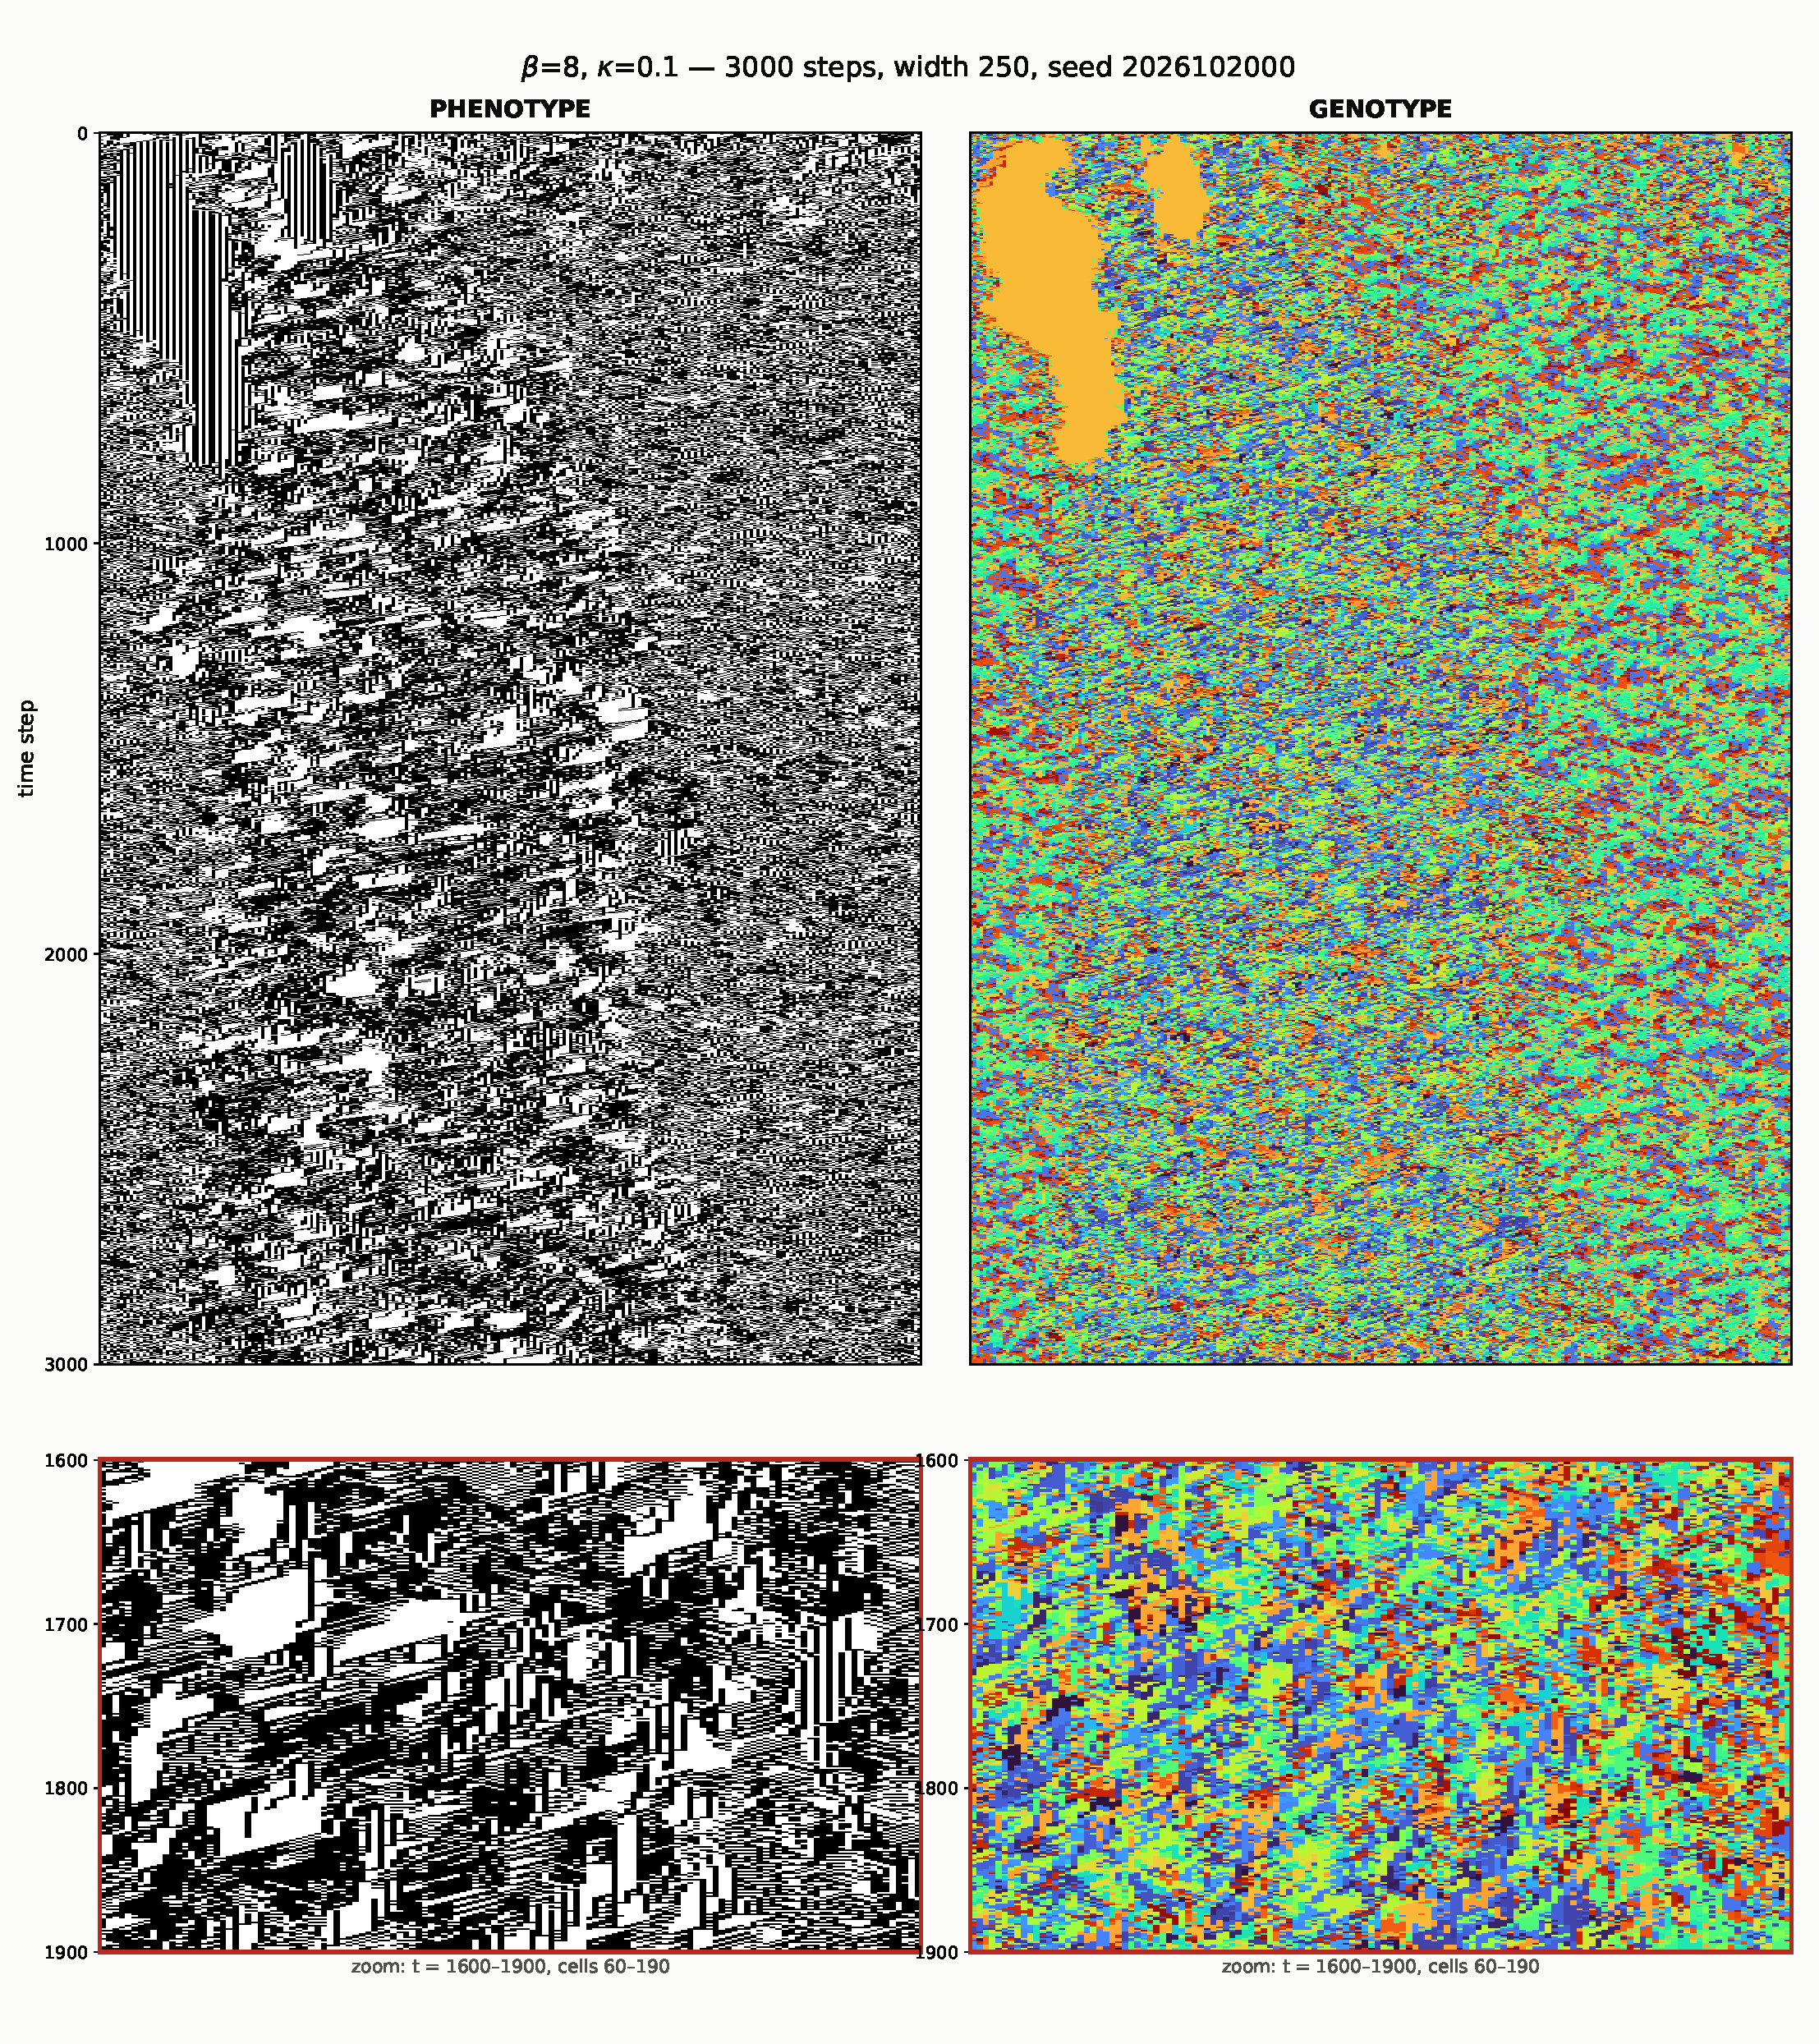
\includegraphics[width=\linewidth]{figures/exo-lavalamp-spacetime.pdf}
\caption{$\beta = 8$, $\kappa = 0.1$, both layers. Coherent diagonal propagating
structure runs the full sheet after the initial transient. The genotype carries
one monoculture region, gone by $t \approx 500$, and thereafter remains diverse
(mean row diversity $0.306$, churn $0.405$ per step, all $256$ sigils present).
The lower row zooms to the scale of the frozen regions, median $4$ cells by $24$
steps.}
\label{fig:exo-lavalamp}
\end{figure}

This configuration is the edge of chaos that the paper's opening example
first showed: frozen and moving structure coexisting, neither absorbing the
other---the thing such a search would have been built to find. It is also the one the objective ranks eighth of thirty-five, at
$0.453$, below both arms of its own ridge.

\subsection{The parameters do not determine which phase wins}

The honest description of this region is not that neither phase wins. It is that
\textbf{the parameters do not determine which phase wins.} The second seed at
$\beta = 8$ loses its frozen phase entirely, reading $0.103$, $0.000$ and
$0.001$ across the same three windows. At $\beta = 10$ the two seeds reach
\emph{opposite} outcomes: one sheds its frozen phase to $0.141$, the other
freezes completely and absorbs at $t = 6346$. Widening the lattice to $1000$
cells changes the answer again, and since that run also extended the horizon we
cannot attribute the change to width alone.

Realisation-to-realisation variance dominating a parameter's effect is what a
critical region looks like, and we report it as that rather than as a regime.
What the three examples establish is that this substrate contains configurations
of all three kinds --- one phase winning, the other winning, and neither winning
within the horizon we can afford --- and that they are separated by a bisectable
boundary in $\beta$. What they do not establish is a critical point, which would
require the intermediate behaviour to be a property of the parameters rather than
of the draw, and we have evidence against that at the two points tested.

\begin{figure}[htbp]
\centering
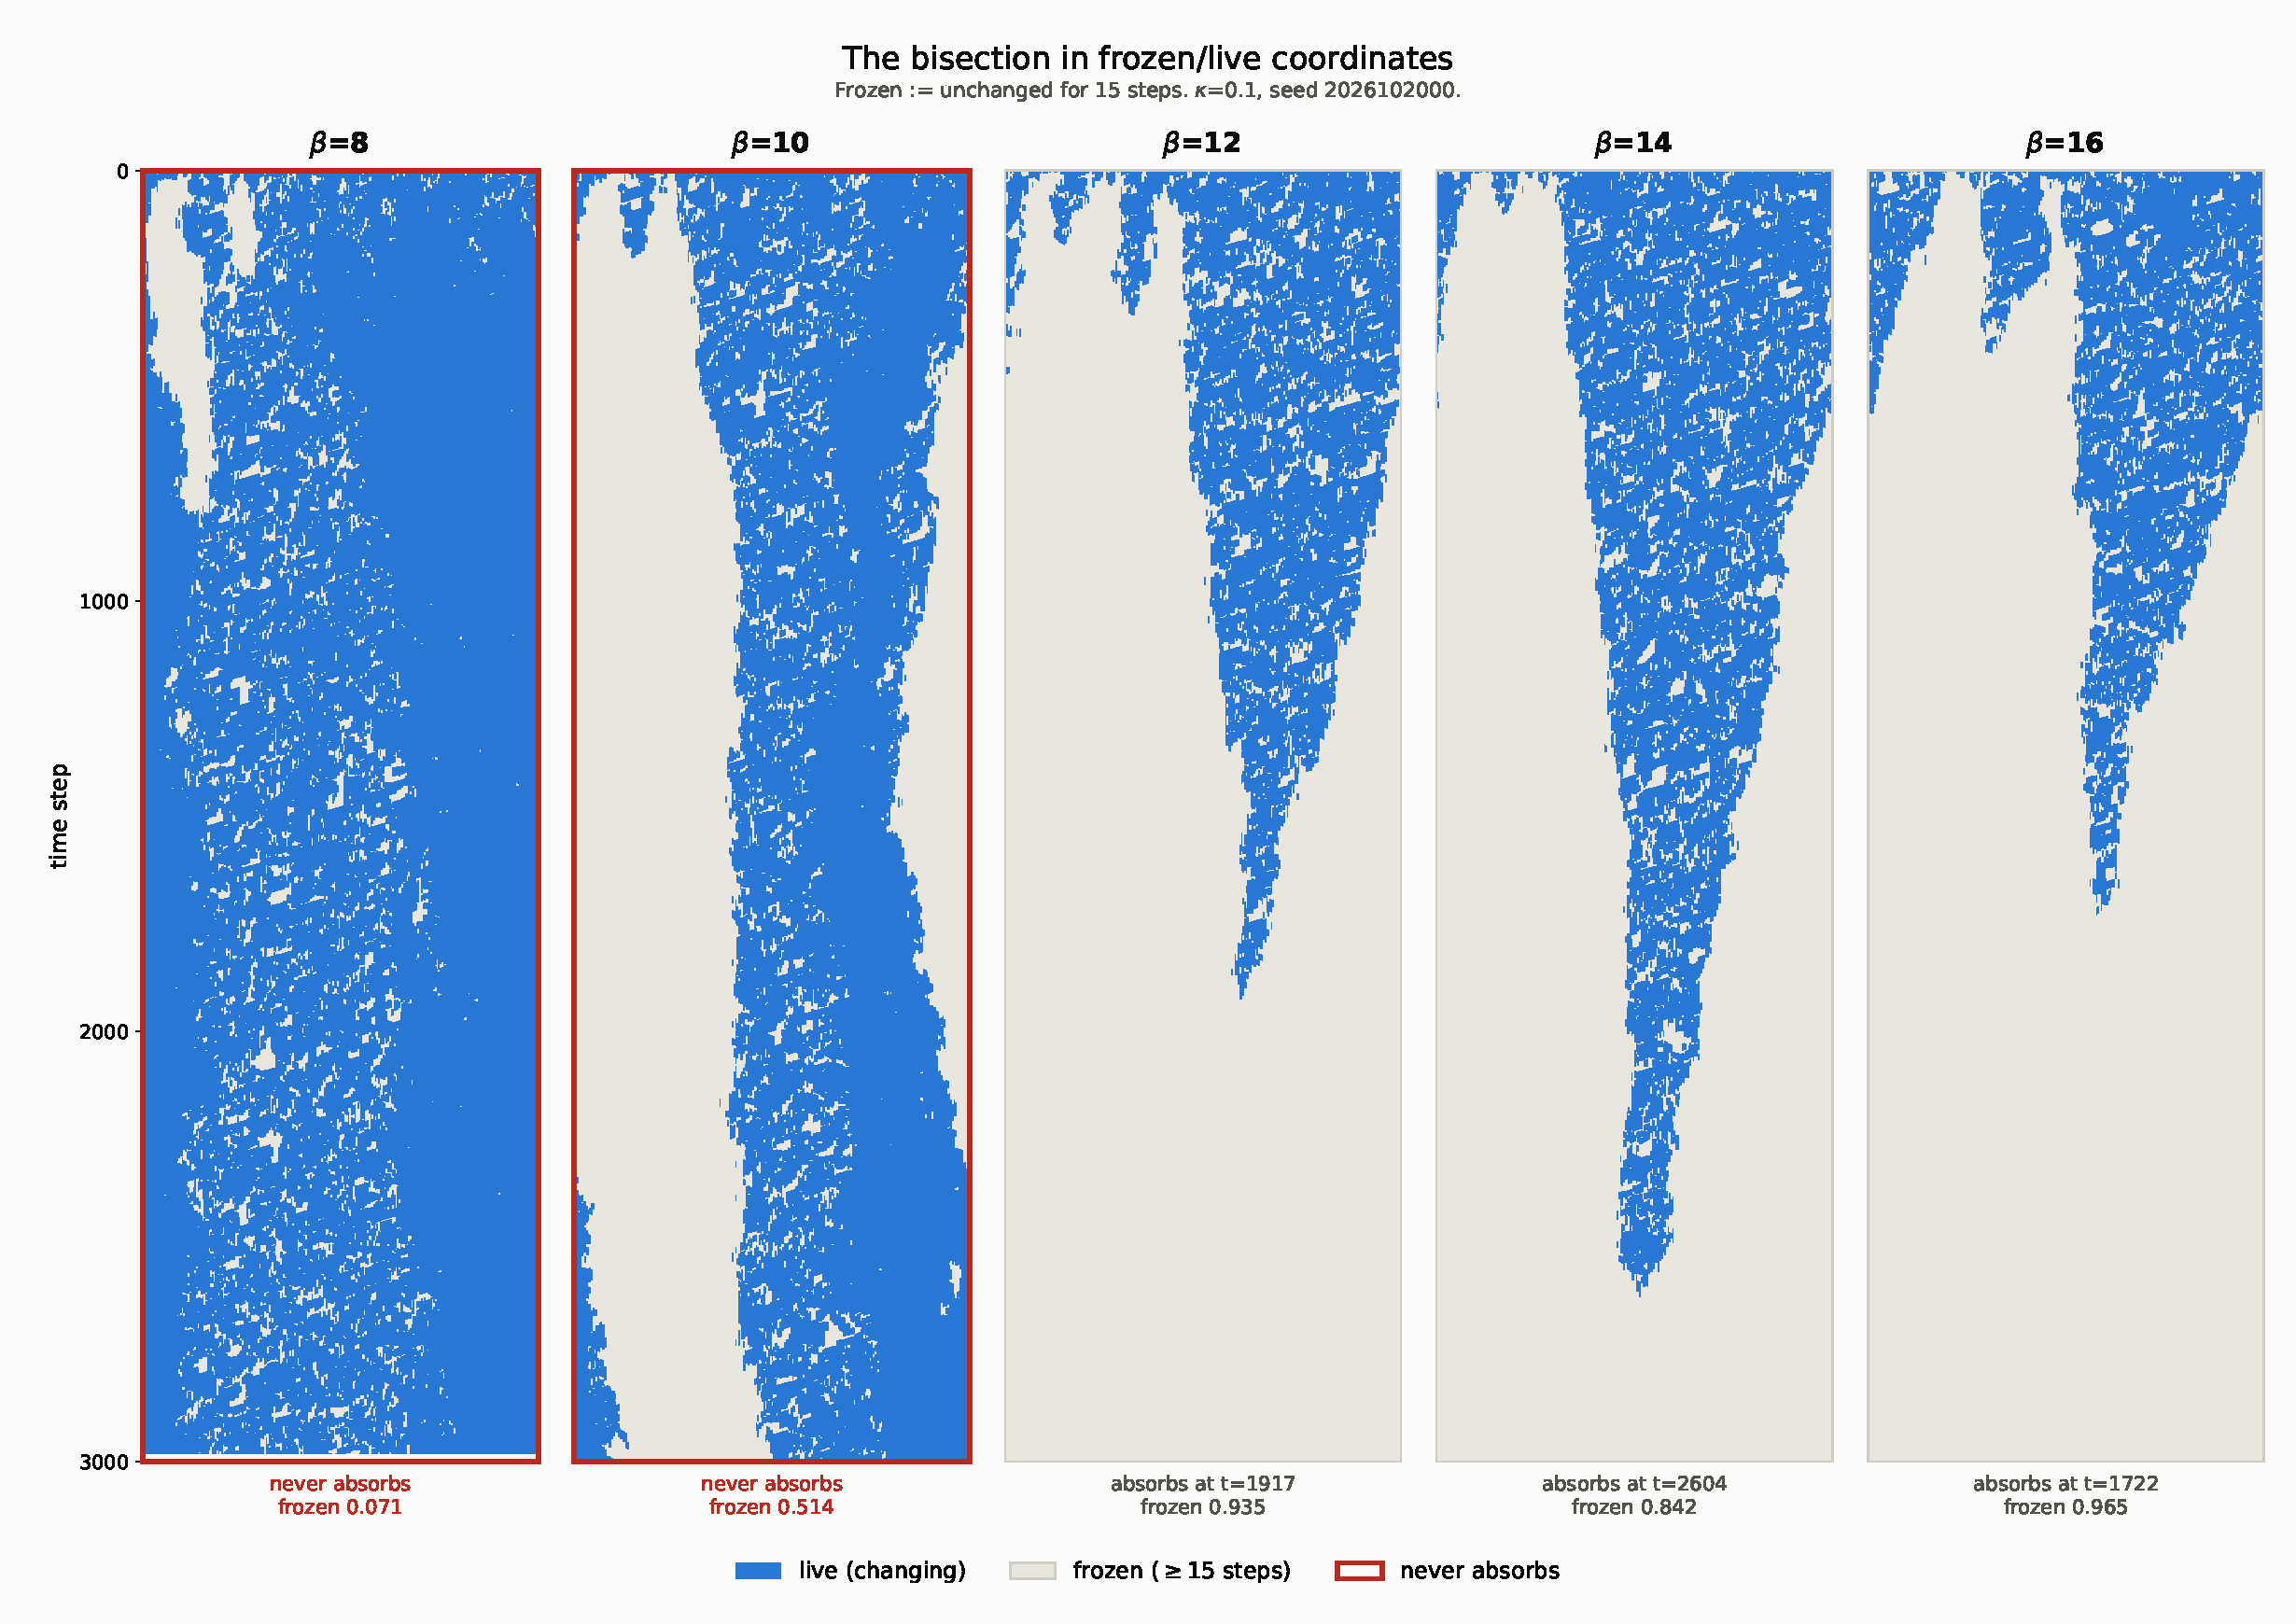
\includegraphics[width=\linewidth]{figures/exo-bisection.pdf}
\caption{The bisection in frozen/live coordinates, $\kappa = 0.1$. Frozen is
defined as unchanged for fifteen steps; at a four-step threshold the median
frozen episode is itself four steps and the turnover count inflates
thirteen-fold. $\beta = 12$, $14$ and $16$ taper to an absorbing state;
$\beta = 8$ and $10$ do not.}
\label{fig:exo-bisection}
\end{figure}

One methodological point generalises beyond these three examples and
dictates the section's use of persistence, rather than a short-window score,
as its measure. Every configuration reported here was present in the
thirty-five-configuration parameter sweep reported in Supplement~4 and was scored there over a $250$-step
window. At that horizon the example in the valley is unremarkable and the arm
that dies looks best. The behaviour that separates them --- absorption at
$t = 1046$, turnover sustained past $t = 9500$ --- occurs entirely outside the
window in which the objective was computed. An instrument validated on
$250$-step reference automata can be measuring a transient in a system whose
transients run four times longer.

\section{No Tested Local Quantity Finds Coexistence, and the Policy Creates the Absorbing States}
\label{sec:exotype-question}

Four deterministic measurements close the question posed in
\secref{sec:exotype-intro}. It separates into two parts---whether a cell can decide
from its own observations where the system should operate (search), and
whether a local rule can keep it there once placed (holding)---and both parts
close negatively.

\emph{The search half was external.} The search that located the examples
is described in Supplement~4: it swept a
thirty-five-cell grid over the selection rule's two parameters at four seeds
per cell, scored each run after the fact, moved over the resulting surface
under a learned surrogate, and restarted after every absorbed probe. None of
those operations is available to a cell inside a run, and the information
they produce arrives once per run rather than once per update decision. The
local substitute a within-run search would need---a cell ranking two
operators by a windowed observation of its own neighbourhood---fails at every
window length:
across eight seeds of the fixed-operator lattice the probability of a correct
pairwise ranking peaks at $0.571$ and \emph{decays} as the window grows, and
the comparison a cell can actually make, against its own neighbour, never
exceeds $0.540$.

The mechanism is a timescale mismatch. The frozen field---using the preceding section's definition, a site is frozen after fifteen unchanged phenotype steps---decorrelates at a site in about six steps, less than half the window
that gives the observable its discriminative power, so integration pools evidence
across contexts that no longer obtain---a fast decision fails by variance, a
slow one by staleness, and no decision rate exists at which feedback through a
temporally integrated detector works. The run-level result---that halting share and change rate predict local compressibility with held-out $R^2 = 0.73$---is unchanged; what fails is per-decision use.

\emph{The holding half is also negative within this family, with a reversal}
(Figure~\ref{fig:interventions}). The natural local mechanism---let cells that
sit in a pure neighbourhood, all frozen or all live, copy the operator of a
cell at a phase boundary, so that the mixed condition invades the pure---was
run at $\beta = 16$, $\kappa = 0.1$ the arm of the ridge that freezes solid.
It froze on all six seeds, and on five of the six \emph{earlier} than the
unmodified policy, by $297$ steps on average: at high precision the operators
found at boundaries are the freeze front's own, so boundary-directed copying
accelerates the phase it was built to resist. For the random-write intervention, each cell receives a fixed intervention interval sampled uniformly from 15 to 25 steps and a random phase offset; we call that interval its \emph{dwell}. When the interval elapses while the cell is in a pure neighbourhood, the cell receives one random operator write. This prevents absorption on all six seeds, but so does the same number of writes applied to uniformly random cells, to within seed noise, so the placement carries nothing. What either
preserves is a foam: small frozen islands, median width $2$ with the
majority at two cells or fewer, surrounded by changing sites, at a frozen
fraction near $0.3$ against the valley configuration's $0.08$ at the same
seed. Whether that state differs
from the valley configuration in \emph{structure} is not settled by the
statistics we computed: the coarse connected regions visible in
Figure~\ref{fig:exo-lavalamp} are a property of its spacetime components,
and under the per-step run-width statistic used here the valley runs measure
median $1$--$2$ as well. Undirected rule noise keeps this lattice alive; we
do not claim it keeps it at, or away from, the found configuration. A
complementary intervention targets the phase-boundary cells instead
(Figure~\ref{fig:interventions}, bottom row): at matched dose its outcome is
indistinguishable from its count-matched random-placement control, and at low dose it drives
the lattice to a near-frozen state threaded by one persistent changing seam
--- the write rate, not the placement, sets the outcome.

\begin{figure}[htbp]
\centering
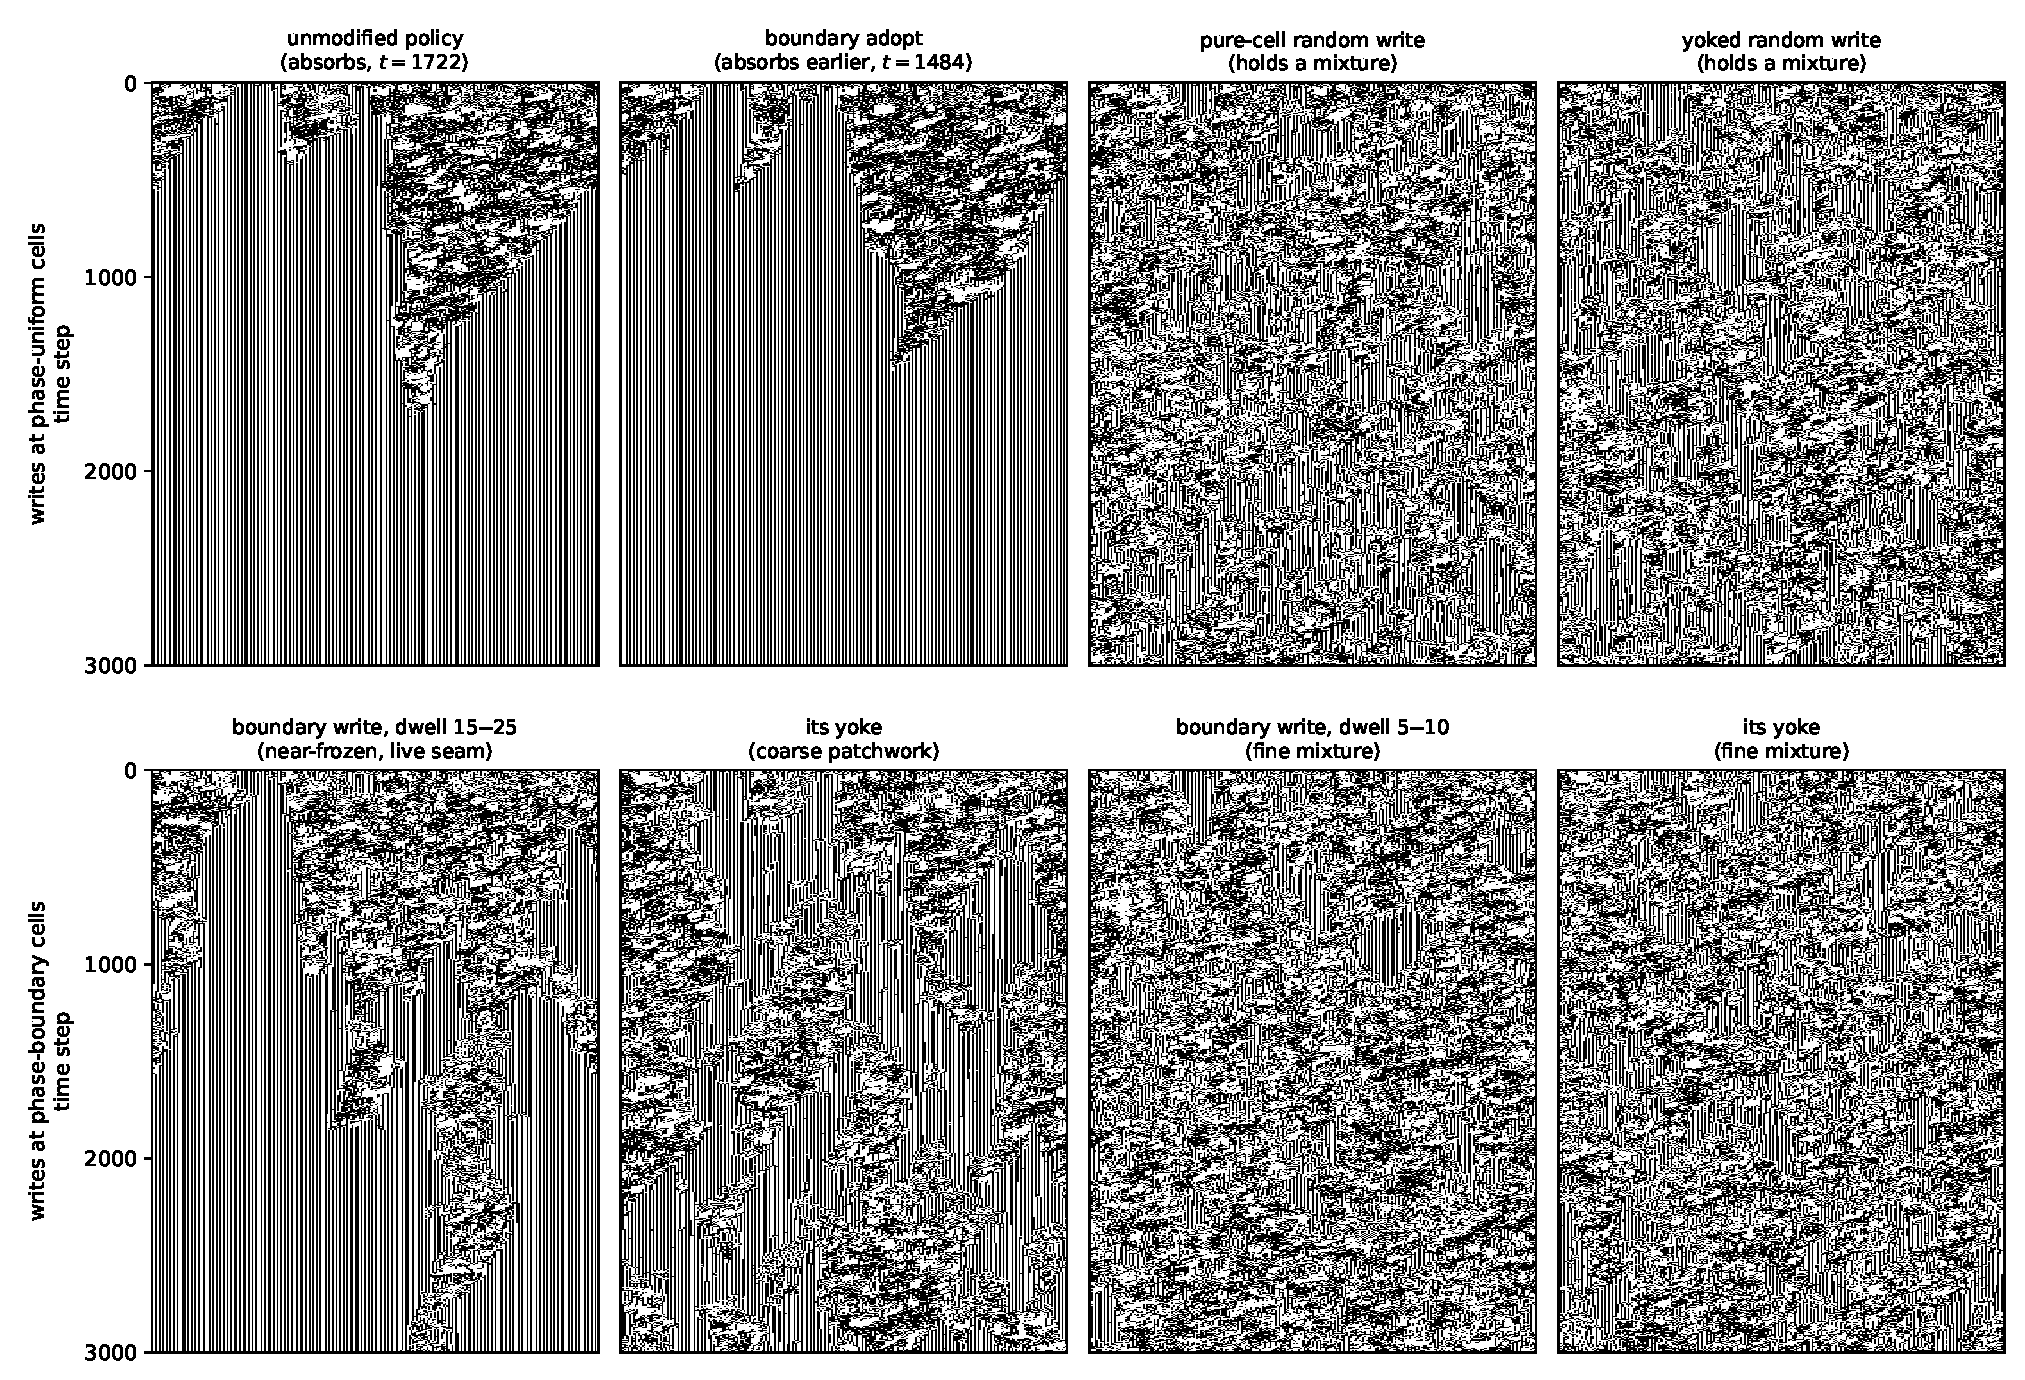
\includegraphics[width=\linewidth]{figures/interventions.pdf}
\caption{\textbf{Two local interventions at the freezing arm.} $\beta = 16$,
$\kappa = 0.1$, seed $2026102000$, whose unmodified-policy run is the absorbing $\beta=16$ example in Figure~\ref{fig:exo-bisection}; phenotype
spacetimes, all runs from identical initial conditions, frozen defined as
unchanged for fifteen steps. \emph{Top row}, writes at phase-uniform cells:
the unmodified selection policy absorbs at $t = 1722$; boundary-directed
adoption---cells in uniform surroundings copying the operator of a cell at a
phase boundary---absorbs \emph{earlier}, at $t = 1484$; one random operator
write per dwell at such cells prevents absorption, and so does the same
number of writes at uniformly random cells (median frozen-run width $2$,
frozen fraction near $0.3$ for both; across six seeds the pair is
statistically indistinguishable). \emph{Bottom row}, writes at
phase-boundary cells: at dwell $15$--$25$ the lattice approaches a frozen
state threaded by a persistent changing seam, while its count-matched yoke
holds a coarse patchwork; at dwell $5$--$10$ both arms hold a fine mixture.
Dose, not placement, sets the outcome at matched dose; at low dose the
boundary rule concentrates its writes on the remaining seam.}
\label{fig:interventions}
\end{figure}

\emph{A control changes what the question presupposes.} In the first no-adoption control, six runs use the same initial conditions as the six absorbing runs above, but the randomly assigned operators remain fixed; none freezes solid or dies out, and their frozen fractions remain between $0.083$ and $0.145$ through the full horizon. In a second no-adoption control at width $120$, all twenty-four runs likewise retain both changing and frozen sites, including runs begun from a deliberately frozen-leaning state. Within the tested
configuration family, then, freezing solid is an effect of the adoption rule
at high precision, not a behaviour of the lattice underneath: switch adoption
off and the same lattices, from the same starting points, hold a mixture
through the full horizon. The bisection that located the examples sits at a
different level entirely---it varied the rule's precision from outside,
between runs, and acted within none of them; it was a search tool, and this
control is what separates what it found from what the rule it varied does at
its extreme setting. Two boundaries on this statement matter.
First, its scope is thirty runs, two geometries, and one vocabulary of twelve operators; it is not a claim about rule-rewriting lattices generally.
Second, the uncontrolled state has not been shown to match the found
configuration in structure---the statistic that would separate or identify
them is not among those we computed. What the control establishes is
narrower: in this family, absorption is a property of running the selection
policy at high precision, not of the substrate the policy acts on.

\section{Two Probes from the Literature: the Freeze Is Nucleation-Limited, and a One-Sided Rule Holds a Mixture}
\label{sec:probes}

The related-work audit left two readings of Part~III open, and both are
directly testable. First, when a substrate co-evolves with the state on it,
a continuous absorbing transition classically becomes first order, with
bistability and hysteresis \parencite{gross2006epidemic}---a reading on
which the freezing of \secref{sec:exotype-question} is one branch of a bistable
pair rather than the endpoint of a crossover. Second, the one local design
class our interventions did not test is the asymmetric rule of
\textcite{droste2013analytical}: tentative while no information is
available, decisive on one-sided evidence.

The first reading is supported, in a specific form: the freeze is
\emph{nucleation-limited}. An adiabatic sweep of $\beta$ upward through the
freezing regime and back ($2{,}500$ steps per plateau, six seeds) produced
no freezing at any $\beta$ up to $32$ once the lattice had developed live
churn, and an extended dwell---$10{,}000$ steps at $\beta = 16$, six times
the cold-start absorption time---produced none either: transient settled
islands stayed below $3\%$ of the lattice and dissolved. Yet the same
dynamics from a cold start absorbs by $t \approx 1{,}700$ (the pipeline
reproduces \secref{sec:exotype-question}'s pinned-seed absorption to within one
step), and an \emph{established} frozen phase wins: a lattice spliced
half-and-half from an absorbed donor run and a churning donor run, restarted
at $\beta = 16$ with nothing done at the seam, was fully absorbed by the
frozen half in five of six seeds within $5{,}000$ steps. The frozen phase
invades any front it holds but cannot arise from churn at these horizons:
two macrostates persist at identical parameters, selected by the initial
condition, with a critical nucleus somewhere between the largest transient
island ($\sim$$7$ cells) and the spliced domain ($125$ cells). This is the
bistable phenomenology the co-evolving-substrate literature predicts, and it
scopes the crossover result of Part~I in the direction that literature
warns: at tested sizes, absence of a critical point and a
nucleation-limited first-order transition are not distinguishable.

The second reading is also confirmed, and it rescopes one sentence of
\secref{sec:exotype-question}. A cell whose phenotype has been unchanged for
$W^{*}$ steps is one-sided evidence of the frozen phase---live cells occur
in both macrostates and certify nothing. A rule that takes one random
vocabulary write at exactly such cells (refractory $15$ steps; nothing done
anywhere else) prevents absorption on all six seeds at $W^{*} = 100$ using
$0.51$ writes per step across the lattice; its count-matched control, the
same closed-loop write budget at uniformly random cells, needs $6.6$ times
the dose and still carries three times the frozen mass. Placement therefore
carries information once the trigger is one-sided; the earlier finding that
``the placement carries nothing'' is a fact about blind and cadence-triggered
writes, not about local intervention as such. The scope of the positive is
equally sharp: what the one-sided rule holds is a foam finer than the
noise arms' (median frozen-run width $1$; three-quarters of runs at two
cells or fewer; frozen fraction $0.17$), not the found configuration's
extended regions. The negative that stands is unchanged in kind but now
exactly bounded: no tested local quantity \emph{finds} the coexistence
condition, and no tested intervention---symmetric, blind, or
one-sided---recovers the \emph{found configuration}. What fell was only
the claim that local placement cannot matter.
